\subsection{Unpacking the Magic of Isotropic Radiators!}

\begin{tcolorbox}[colback=gray!10, colframe=black, title=E9A01] What is an isotropic radiator? 
\begin{enumerate}[label=\Alph*.]
    \item A calibrated, unidirectional antenna used to make precise antenna gain measurements
    \item An omnidirectional, horizontally polarized, precisely calibrated antenna used to make field measurements of antenna gain
    \item \textbf{A hypothetical, lossless antenna having equal radiation intensity in all directions used as a reference for antenna gain}
    \item A spacecraft antenna used to direct signals toward Earth
\end{enumerate} \end{tcolorbox}

\subsubsection{Related Concepts}

An isotropic radiator is an essential concept in the field of radio communications and antenna theory. To understand what it represents, let us dissect its properties:

1. \textbf{Hypothetical Nature:}: An isotropic radiator does not exist in practical terms; it is a theoretical construct used to simplify the analysis of antenna performance.
2. \textbf{Radiation Intensity:}: It is characterized by having equal radiation intensity in all directions in three-dimensional space, meaning that regardless of the angle at which the antenna is viewed, it radiates the same amount of power.
3. \textbf{Reference for Gain Measurements:}: The isotropic radiator serves as a reference point for measuring the gain of real antennas. Antenna gain is a measure of how well the antenna directs radio frequency energy in a particular direction compared to the isotropic radiator.

To better understand the concept of isotropic radiation, consider how we measure the output of actual antennas. For example, if a particular antenna is said to have a gain of 3 dBi, it indicates that it radiates three times the power in the direction of maximum radiation compared to an isotropic radiator.

\subsubsection{Illustration}

\begin{center}
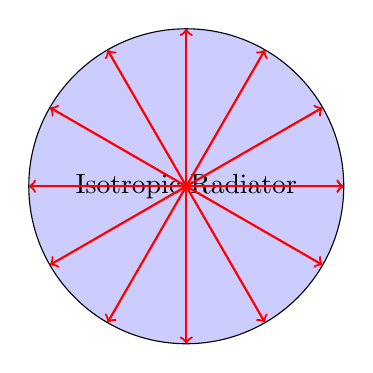
\begin{tikzpicture}
    \filldraw[fill=blue!20] (0,0) circle (2cm);
    \node at (0,0) {Isotropic Radiator};
    \foreach \x in {0,30,...,360} {
        \draw[->, thick, red] (0,0) -- (\x:2);
    }
\end{tikzpicture}
\end{center}

In the above diagram, the isotropic radiator is represented by a circle, and the arrows indicate the equal radiation intensity in all directions, emphasizing its omnidirectional property.

Understanding isotropic radiators is crucial for any further studies in antenna theory and radio communications as it provides a benchmark against which all real antennas are compared. Thus, one must recognize that while isotropic radiators cannot be built physically, they lay the groundwork for practical applications in the field.
